\documentclass[border=6pt]{standalone}
\usepackage[T1]{fontenc}
\usepackage{lmodern}
\usepackage{tikz}
\usetikzlibrary{arrows.meta,positioning,shapes.geometric,calc,fit}
\begin{document}
\hyphenpenalty=10000 \exhyphenpenalty=10000
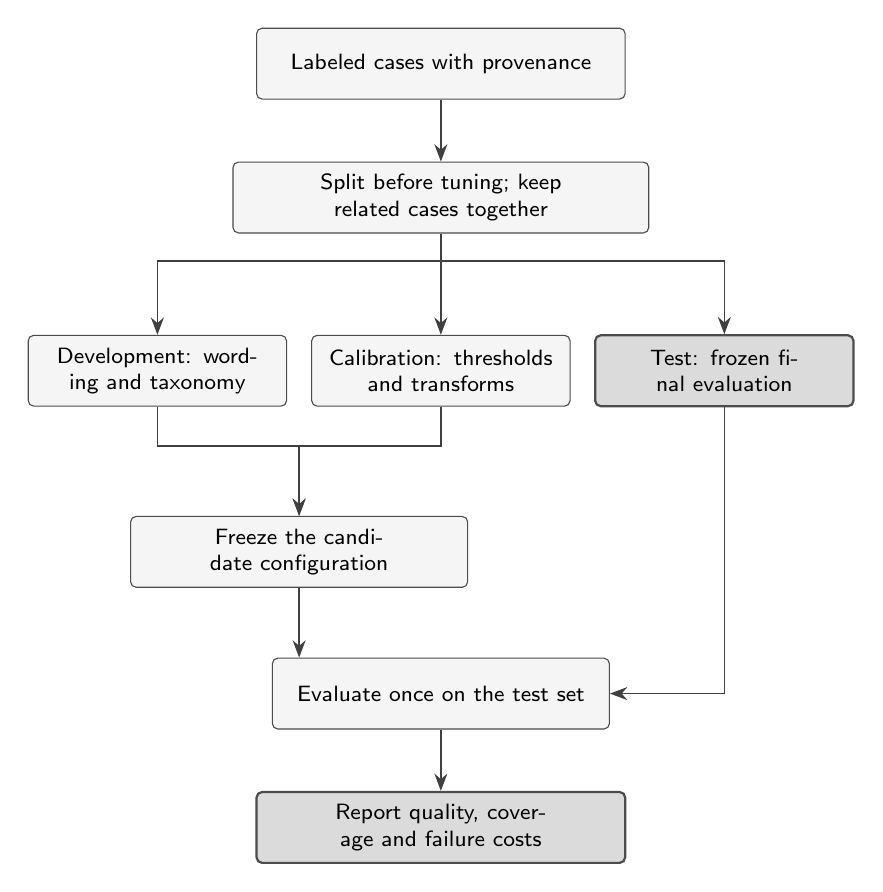
\begin{tikzpicture}[
  font=\footnotesize\sffamily,
  box/.style={draw=black!70, rounded corners=2pt, fill=black!4, align=center,
              text width=3.0cm, minimum height=0.9cm, inner sep=4pt},
  key/.style={box, fill=black!14, line width=0.8pt},
  arr/.style={-{Stealth[length=2.2mm]}, draw=black!75, line width=0.6pt}
]
\node[box, text width=4.4cm] (c) at (0,0) {Labeled cases with provenance};
\node[box, text width=5.0cm] (s) at (0,-1.7) {Split before tuning; keep related cases together};
\node[box] (dev) at (-3.6,-3.9) {Development: wording and taxonomy};
\node[box] (cal) at (0,-3.9) {Calibration: thresholds and transforms};
\node[key] (tst) at (3.6,-3.9) {Test: frozen final evaluation};
\node[box, text width=4.0cm] (f) at (-1.8,-6.2) {Freeze the candidate configuration};
\node[box, text width=4.0cm] (e) at (0,-8.0) {Evaluate once on the test set};
\node[key, text width=4.4cm] (r) at (0,-9.7) {Report quality, coverage and failure costs};

\draw[arr] (c) -- (s);
\draw[arr] (s.south) -- ++(0,-0.35) -| (dev.north);
\draw[arr] (s.south) -- ++(0,-0.35) -| (cal.north);
\draw[arr] (s.south) -- ++(0,-0.35) -| (tst.north);
\draw[arr] (dev.south) -- ++(0,-0.5) -| (f.north);
\draw[arr] (cal.south) -- ++(0,-0.5) -| (f.north);
\draw[arr] (f.south) -- (f.south |- e.north);
\draw[arr] (tst.south) |- (e.east);
\draw[arr] (e) -- (r);
\end{tikzpicture}
\end{document}
